\documentclass[letter, 10pt]{article}
\usepackage[utf8]{inputenc}
\usepackage[spanish]{babel}
\usepackage{amsfonts}
\usepackage{amsmath}
\usepackage[dvips]{graphicx}
\usepackage{url}
\usepackage[top=3cm,bottom=3cm,left=3.5cm,right=3.5cm,footskip=1.5cm,headheight=1.5cm,headsep=.5cm,textheight=3cm]{geometry}
\usepackage{listings}
\usepackage{color}
\usepackage{fancyvrb}
\usepackage{fancyhdr}

\pagestyle{fancyplain}

\lhead{Workshop Taller de Gestión} %Parte superior izquierda
\rhead{\bf \it Tutoriales} %Parte superior derecha
\lfoot{} %Parte inferior izquierda.
\cfoot{} %Parte inferior central
\rfoot{\bf \thepage} %Parte inferior derecha
\renewcommand{\footrulewidth}{0.4pt} %Linea de separacion inferior


\begin{document}

\title{Tutorial Planner}
\author{Rodrigo Fernández \and Cristián Maureira \and Gabriel Zamora\\ \small{\texttt{\{rfernand,cmaureir,gzamora\}@inf.utfsm.cl}}}
%\titlegraphic{
\includegraphics[height=1cm]{img/logos}}
\date{\today}

\maketitle

\section{Qué es Planner}
Planner es una herramienta para planear, programar y seguir proyectos para el
escritorio GNOME. Es una aplicación GTK+ escrita en C y licenciada bajo GPL
(versión 2 o posterior).
\subsection{Características}
Puede almacenar sus datos en ficheros XML o en una base de datos
postgresql. Los proyectos pueden ser impresos en PDF o exportados a HTML para
una visualización simple desde cualquier navegador web.

El programa permite:
\begin{itemize}
    \item Gestión de calendarios
    \item Gestión de recursos
    \item Seguimiento del avance del proyecto
    \item Enlazar tareas
    \item Exportación a diferentes formatos
\end{itemize}
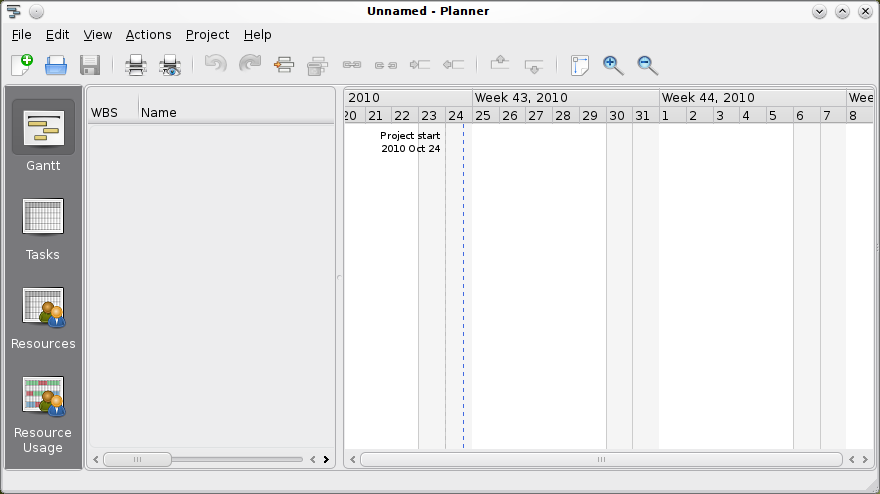
\includegraphics[scale=0.6]{img/planner_1}\\

\section{Instrucciones de uso}
\begin{description}
    \item[Agregar recursos]:
\begin{enumerate}
    \item Click en Resources.
    \item Click derecho y click en "Insert Resource".
    \item Click derecho y click en "Editar Resource".
    \begin{enumerate}
        \item Poner nombre, nombre corto, tipo y costo según sea el caso.
    \end{enumerate}
\end{enumerate}

    \item[Creación de una tarea]:
\begin{enumerate}
    \item Click derecho y click en "Insert Task"
    \item Doble click en la tarea nueva para abrir su edición.
    \begin{enumerate}
        \item Poner nombre, duración.
        \item Asignar recursos.
        \item Indicar predecesores si es ese el caso.
    \end{enumerate}
\end{enumerate}

    \item[Generar pdf]:
\begin{enumerate}
    \item Ir a "File"
    \item Ir a "Print..."
    \item Seleccionar "Output Format: pdf"
    \item Ponerle un nombre al archivo y elegir donde será guardado.
    \item Click en "Print".
\end{enumerate}
    

\item[Recuerda al final guardar el proyecto.]

\end{description}

\section{Ejercicio}
Tomando en consideración los requerimientos de la herramienta, realice una
aproximación de la carta gantt asignando tiempos y recursos correspondientes.
En los recursos, agregue a los miembros de su grupo, y planee la actividad
para el primer mes de trabajo.

\end{document}
